\chapter{Compact Models}
Here we introduce different formulations for the traveling salesman problem that we implemented. For all the following models we will use the decision variable $x_{ij}$ already defined in Section \ref{TSPdef}.\\
According to \cite{ormanWilliams}, we considered the case of the Asymmetric version of the traveling salesman problem, which can be considered more general than the Symmetric version.\\
Main advantage of going with these models, is that once the model is written, it can be solved as a ``black box" by CPLEX solver.\\
To improve the time performance in the computation of the optimal solution, we implemented part of constraints about the subtour elimination through \textit{lazy constraints}. This allowed us to improve the performance of the models because this kind of constraints will be applied only once needed.

\section{Sequential formulation}
For this version, formulated by Miller, Tucker and Zemlin (MTZ) in 1960 \cite{MTZ}, we introduce the continuous variable 
\begin{equation*}
	u_i = \text{sequence in which point i is visited} \ (i \neq 1)
\end{equation*}
and the constraint \ref{eqn:mtz-constraint}.

\begin{subequations}
	\begin{equation}
		\text{min} \underbrace{\sum_{(i,j) \in A} c_{ij}x_{ij}}_\text{circuit cost}
	\end{equation}
	\begin{equation}
		\underbrace{\sum_{(i,j) \in \delta^{-}(j)} x_{ij} = 1}_\text{one edge incoming in j}, \quad j \in V 
		\label{eqn:2.1b}
	\end{equation}
	\begin{equation}
		\underbrace{\sum_{(i,j) \in \delta^{+}(j)} x_{ij} = 1}_\text{one edge outgoing in i}, \quad i \in V
		\label{eqn:2.1c}
	\end{equation}
	\begin{equation}
		u_i-u_j+nx_{ij} \leq n-1 \quad \forall i,j \in N-\lbrace 1 \rbrace, \ i\neq j \;\; \textbf{(Lazy constraint)}
		\label{eqn:mtz-constraint}
	\end{equation}
\end{subequations}

\noindent Constraints \ref{eqn:mtz-constraint} ensure that, if the salesman travels from i to j, then the position of node j is one more than that of node i. This allows to have only a polynomial number of variable and constraints. In total, there are $O(n^2)$ variables and $O(n^2)$ constraints. The problem is no more NP-Hard, but the relaxation of the problem is somewhat weak and as one can see in the section where compact models are compared, it yields to decent performances only for small instances.

\section{Flow-based formulations}

\subsection{Single commodity flow}
Provided by Gavish and Graves in 1978 \cite{gavish_travelling_1978}, it adds continuous variables: 
\begin{equation*}
	y_{ij} = \text{flow in arch} \ (i,j) \ i \neq j
\end{equation*}
%In total it has $n(n+2)$ constraints, $n(n-1)$ 0-1 variables and $n(n-1)$ continuous variables.

\begin{subequations}
	\begin{equation}
		\text{min} \sum_{(i,j) \in A} c_{ij}x_{ij} \\
	\end{equation}
	\begin{equation}
		\sum_{(i,j) \in \delta^{-}(j)} x_{ij} = 1, \quad j \in V \\
	\end{equation}
	\begin{equation}
		\sum_{(i,j) \in \delta^{+}(j)} x_{ij} = 1, \quad i \in V \\
	\end{equation}
	\begin{equation}
		y_{ij} \leq (n-1)x_{ij} \quad \forall i,j \in N, \ i \neq j \\
	\end{equation}
	\begin{equation}
		\sum_{j, \; j \neq 1} y_{1j} = n-1 \;\; \textbf{(Lazy constraint)}\\
	\end{equation}
	\begin{equation}
		\sum_{i, \; i \neq j} y_{ij} - \sum_{k, \; i \neq k} y_{jk} = 1 \quad \forall j \in N - \lbrace 1 \rbrace
	\end{equation}
\end{subequations}

\noindent The idea is that whenever one node is chosen, the salesman delivers one unit of commodity flow. In this way, an order between the nodes is picked and subtours are impossible.\\
This formulation has $O(n^2)$ variables and $O(n)$ constraints. The relaxation of the linear problem works better than the MTZ, as one can observe in the section about the comparison between the compact models.

\subsection{Two commodity flow}
Created by Finke, Claus and Gunn in 1983. It maintains constraint \ref{eqn:2.1b} and \ref{eqn:2.1c} (from this point they and the objective function will not be shown in the formulation) and introduce the continuous variables:
\begin{equation*}
	y_{ij} = \text{flow of commodity 1 in arc} \ (i,j) \ i \neq j
\end{equation*}
\begin{equation*}
	z_{ij} = \text{flow of commodity 2 in arc} \ (i,j) \ i \neq j
\end{equation*}
and add the constraints:

\begin{subequations}
	\begin{equation}
	\label{eqn:f2-const-1}
	 	\sum_{j, \; j \neq 1} (y_{1j}-y_{j1}) = n-1 \;\; \textbf{(Lazy constraint)}
	\end{equation}
	\begin{equation}
	\label{eqn:f2-const-2}
		\sum_{j} (y_{ij}-y_{ji}) = 1 \quad \forall i \in N-\lbrace 1 \rbrace, \ i \neq j
	\end{equation}
	\begin{equation}
	\label{eqn:f2-const-3}
		\sum_{j, \; j \neq 1} (z_{1j}-z_{j1}) = -(n-1) \;\; \textbf{(Lazy constraint)}
	\end{equation}
	\begin{equation}
	\label{eqn:f2-const-4}
		\sum_{j} (z_{ij}-z_{ji}) = -1 \quad \forall i \in N-\lbrace 1 \rbrace, \ i \neq j
	\end{equation}
	\begin{equation}
	\label{eqn:f2-const-5}
		\sum_{j} (y_{ij}+z_{ij}) = n-1 \quad \forall i \in N
	\end{equation}
	\begin{equation}
	\label{eqn:f2-const-6}
		y_{ij}+z_{ij} = (n-1)x_{ij} \quad \forall i, j \in N
	\end{equation}
\end{subequations}

%In total it has $n(n+4)$ constraints, $n(n-1)$ 0-1 variables and $2n(n-1)$.
\noindent Constraints \ref{eqn:f2-const-1} and \ref{eqn:f2-const-2} force $(n-1)$ units of commodity 1 to flow into city 1 and 1 unit of commodity to flow out from every other node.\\
Constraits \ref{eqn:f2-const-3} and \ref{eqn:f2-const-4} force $(n-1)$ units of commodity 2 to flow out from city 1 and 1 unit of commodity to flow into every other node.\\
Constraints \ref{eqn:f2-const-5} force exactly $(n-1)$ units of commodity in each arc and constraints \ref{eqn:f2-const-6} only allow flow in an arc if present.\\
The formulation has $O(n^2)$ constraints and $O(n^2)$ variables.

\subsection{Multi-commodity flow}
Proposed by Wong and Claus in 1984. Again constraint \ref{eqn:2.1b} and \ref{eqn:2.1c} are maintained. It introduce the continuous variable:
\begin{equation*}
	y_{ij}^k = \text{flow of commodity k in arc} \ (i,j) \in N-\lbrace 1 \rbrace
\end{equation*}
and the following constraints:
\begin{subequations}
	\begin{equation}
	\label{eqn:fm-const-1}
		y_{ij} \leq x_{ij} \quad \forall i,j,k \in N, \ k \neq 1
	\end{equation}
	\begin{equation}
	\label{eqn:fm-const-2}
		\sum_{i} y_{1i}^k = 1 \quad \forall k \in N-\lbrace 1 \rbrace
	\end{equation}
	\begin{equation}
	\label{eqn:fm-const-3}
		\sum_{i} y_{i1}^k = 0 \quad \forall k \in N-\lbrace 1 \rbrace
	\end{equation}
	\begin{equation}
	\label{eqn:fm-const-4}
		\sum_{i} y_{ik}^k = 1 \quad \forall k \in N-\lbrace 1 \rbrace
	\end{equation}
	\begin{equation}
	\label{eqn:fm-const-5}
		\sum_{j} y_{kj}^k = 0 \quad \forall k \in N-\lbrace 1 \rbrace
	\end{equation}
	\begin{equation}
	\label{eqn:fm-const-6}
		\sum_{i} y_{ij}^k - \sum_{i} y_{ji}^k = 0 \quad \forall j,k \in N-\lbrace 1 \rbrace, \ j \neq k
	\end{equation}
\end{subequations}
%In total there are $n^3+n^2+6n-3$ constraints, $n(n-1)$ 0-1 variables and $n(n-1)^2$
Constraints \ref{eqn:fm-const-1} only allow flow in an arc which is present. Constraints \ref{eqn:fm-const-2} force exactly one unit of each commodity to flow into city 1 and constraints \ref{eqn:fm-const-3} does the opposite, preventing commodity to flow out from city 1.\\
Constraints \ref{eqn:fm-const-4} force exactly one unity of commodity k to flow out from city k and constraints \ref{eqn:fm-const-5} prevent any of commodity k flowing into city k.\\
Finally, constraints \ref{eqn:fm-const-6} force balance for all commodities at each node, apart from city 1 and for commodity k at city k.\\
There is a total number of $O(n^3)$ constraints and $O(n^2)$ variables.

\section{Time staged formulations}

We decided also to explore this section of compact models, exploiting CPLEX's solver that just requires the models to be written. Dealing with performance, especially the T1 and T2 were not working good in practice and required too much to compute the optimal solution.

\subsection{First stage dependent}
Introduced by Fox, Gavish and Graves in 1980. Constraint \ref{eqn:2.1b} and \ref{eqn:2.1c} are maintained, in addition we have 0-1 integer variables:
\[ y_{ij}^t =
	\begin{cases}
		1 \quad \text{if the edge} \ (i,j) \ \text{is traversed at stage t} \\
		0 \quad \text{otherwise}
	\end{cases}
\]
and constraints below, for a total of $n(n+2)$ constraints and $n(n-1)(n+1)$ 0-1 variables.

\begin{subequations}
	\begin{equation}
		\sum_{i,j,t} y_{ij}^t = n
	\end{equation}
	\begin{equation}
		\sum_{j,t \; t \geq 2} ty_{ij}^t - \sum_{k,t} ty_{ki}^t = 1 \quad \forall i \in N-\lbrace 1 \rbrace 
	\end{equation}
	\begin{equation}
		x_{ij}-\sum_{t} x_{ij}^t = 0 \quad \forall i,j \in N, \ i \neq j
	\end{equation}
	with the condition
	\begin{equation}
		y_{il}^t = 0 \; \forall t \neq n, \quad y_{ij}^t = 0 \; \forall t \neq 1, \quad y_{ij}^l = 0 \; \forall i \neq 1, \quad i \neq j
	\end{equation}
\end{subequations}

\subsection{Second stage dependent}
Provided by Fox, Gavish and Graves in 1980. It uses the same variables of first stage and constraints \ref{eqn:2.1b} and \ref{eqn:2.1c} and it adds:

\begin{subequations} 
	\begin{equation}
		\sum_{i,t \; i \neq j} y_{ij}^t = 1 \quad \forall j \in N
	\end{equation}
	\begin{equation}
		\sum_{j,t \; j \neq i} y_{ij}^t = 1 \quad \forall i \in N
	\end{equation}
	\begin{equation}
		\sum_{i \; j \neq i} y_{ij}^t = 1 \quad \forall t \in N
	\end{equation}
	\begin{equation}
		\sum_{j,t \; t \geq 2} ty_{ij}^t - \sum_{k,t} ty_{ki}^t = 1 \quad \forall i \in N-\lbrace 1 \rbrace \;\; \textbf{(Lazy constraint)}
	\end{equation}
\end{subequations}
In totals there are $4n-1$ constraints and $n(n-1)(n+1)$ 0-1 variables.

\subsection{Third stage dependent}
Again we have the same variables of first stage and constraints \ref{eqn:2.1b} and \ref{eqn:2.1c}. In addition, 
for a total of $2n^2-n+3$ constraints and $n(n-1)(n+1)$ 0-1 variables we have:
\begin{subequations}
	\begin{equation}
		\sum_{j} y_{1j}^1 = 1
	\end{equation}
	\begin{equation}
		\sum_{i} y_{i1}^n = 1
	\end{equation}
	\begin{equation}
		\sum_{j} y_{ij}^t - \sum_{k} y_{ki}^{t-1} = 0 \quad \forall i,t \in N-\lbrace 1 \rbrace
	\end{equation}
\end{subequations}
\newpage
\section{Final comparison between Compact Models}
As explained in the previous sections, we decided mainly to focus on MTZ and Flow Based formulations, because of the time required to compute the optimal solution for the dataset we used.\\
We tested these algorithms on dataset made of instances with a number of nodes up to 80. For bigger instances, the computation of an optimal solution became unfeasible.\\
The instances we used to test all our implementations, from compact models to heuristic algorithms, are taken from the TSPLIB \cite{tsplib}. \\
From our results shown in Figure \ref{fig:compacts10} and \ref{fig:compacts200}, we observed that FLOW1 outperformed the other algorithms. Decent results were obtained also with MTZ and FLOW2. In our implementation, FLOW3 had poor performances.

\begin{figure}[H]
\centering
	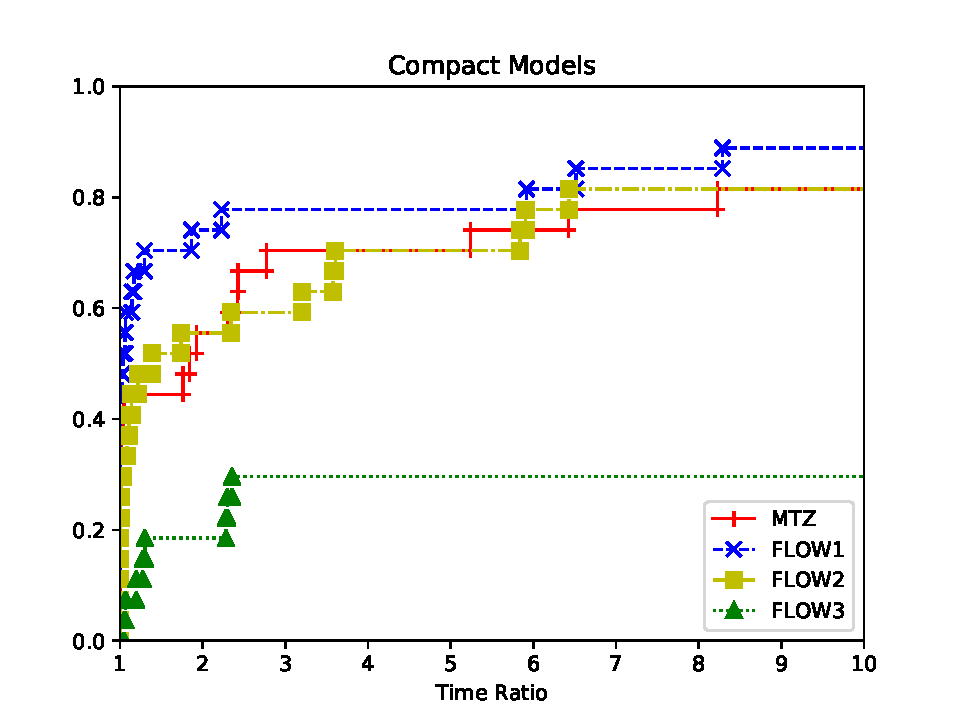
\includegraphics[scale=0.9]{media/compact10.pdf} \\
	\caption{Performance profile for compact models with time ratio 10}
	\label{fig:compacts10}
\end{figure}

\begin{figure}[H]
\centering
	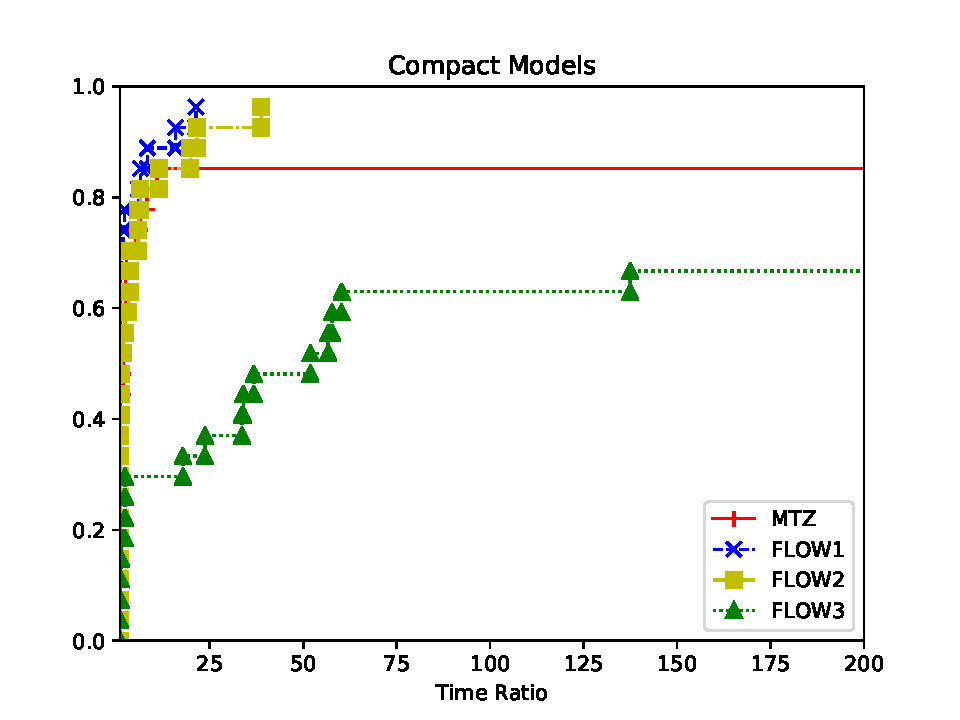
\includegraphics[scale=0.9]{media/compact200.pdf} \\
	\caption{Performance profile for compact models with time ratio 200}
	\label{fig:compacts200}
\end{figure}



